\chapter{Routing}

Routing determine the ``good''\footnote{The minimum path typically} path (
sequence of routers) thru network from source to destination.
Routing protocols use graphs as a mathematical abstraction.

\section{Typologies of routing}

Routing can be \textbf{global}, \textbf{decentralized}, \textbf{static} (where
the route change slowly over time) and \textbf{dynamic} (where the routes change
quickly over time).

\subsection{Global routing}

In this kind of routing routers have the complete topology of the network, with
information about links cost.
Characteristics:
\begin{itemize}
\item ``link state'' algorithm
\item efficent but not faseable
\end{itemize}

An example of a global routing algorithm is the one made by Dijkstra.

\subsubsection{Dijkstra's algorithm}

In this algorithm, that's iterative, all the nodes know link cost between each
other. Basically, it computes least cost path from one note to all the others.

\begin{figure}[t]
  \captionsetup{singlelinecheck=off}
  \centering
  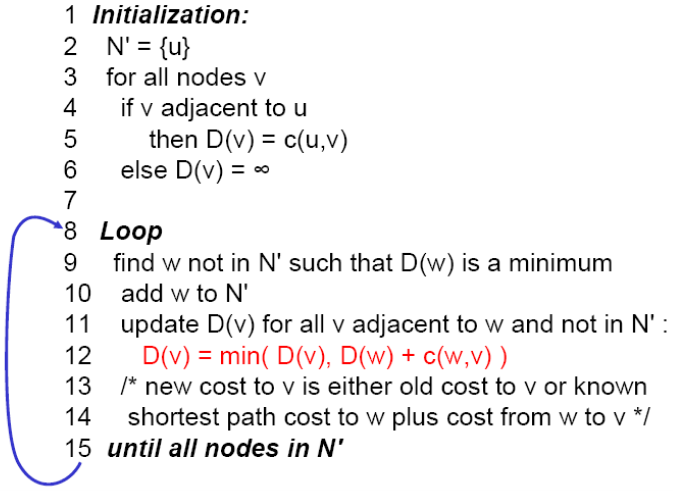
\includegraphics[scale=0.45]{DijkstraAlgo}
  \caption[Dijkstra's algorithm]{Dijkstra's algorithm. Notation:
    \begin{itemize}
    \item $c(x, y)$: link cost from node $x$ to $y$. It's $\infty$ if not direct
      neighbors
    \item $D(v)$: current value of cost of path from source to destination $v$
    \item $p(v)$: predecessor node along path from source to $v$
    \item $N'$: set of nodes whose least cost path definitively known
    \end{itemize}
  }
\end{figure}

\subsection{Decentralized routing}
In this type of routing routers know physically-connected neighbors, and link
cost to them. There is a iterative process of computation and exchange of
information with neighbors.
This algorithms are defined as ``distance vector'' algorithms.

\subsection{Routing based on network typology}

There are different types of routing based on different types of networks.

\paragraph*{Infrastructure based} In this case routing is relatively simple.
There is just a simgle hop from the access point (AP) to the wireless node.

\paragraph*{MANET} Also know as ad-hoc, it has the following characteristics:
\begin{itemize}
\item the network costantly changes
\item wireless nodes are not necessarily all adjacent, so data forwarding
  could be necessary
\end{itemize}
Additionally, there are other difficulties, such as energy consumption and
limited bandwidth (due exchange of routing information) on mobile systems. In
wireline networks we have symmetric links, limited redundancy and fixed
typology, insteas in wireless has asymmetric links, random redundancy with
unplanned, dynamic links. With all this pecurialities, traditional routing
algorithms for MANETS\footnote{MANET stands for \textit{Metropolitan Area
    Network}} are inefficent, and the new one must rely on data link
information, not just network layer updates\footnote{Layer updates only
  determine connectivity}, without using in centralized approaches because they
just don't work. In MANETS nodes can be routers, and they can send different
type of messages between them.
\subparagraph*{Messages classification} There are different type of messages:
\begin{itemize}
\item Unicast: trasmission 1 to 1. In order to achieve a good unicast routing
  protocol there are some goals:
  \begin{itemize}
  \item minimal control overhead
  \item multi-hop path routing capability
  \item no loops
  \end{itemize}
\item Multicast: transmission 1 to N: different receivers of the same message,
  that it can follow different paths
\item Broadcast: transmission 1 to N: everyone receives the message
\end{itemize}

\section{Protocols classification}
% TODO later as is a long part
